\begin{figure}[t]
    \centering
    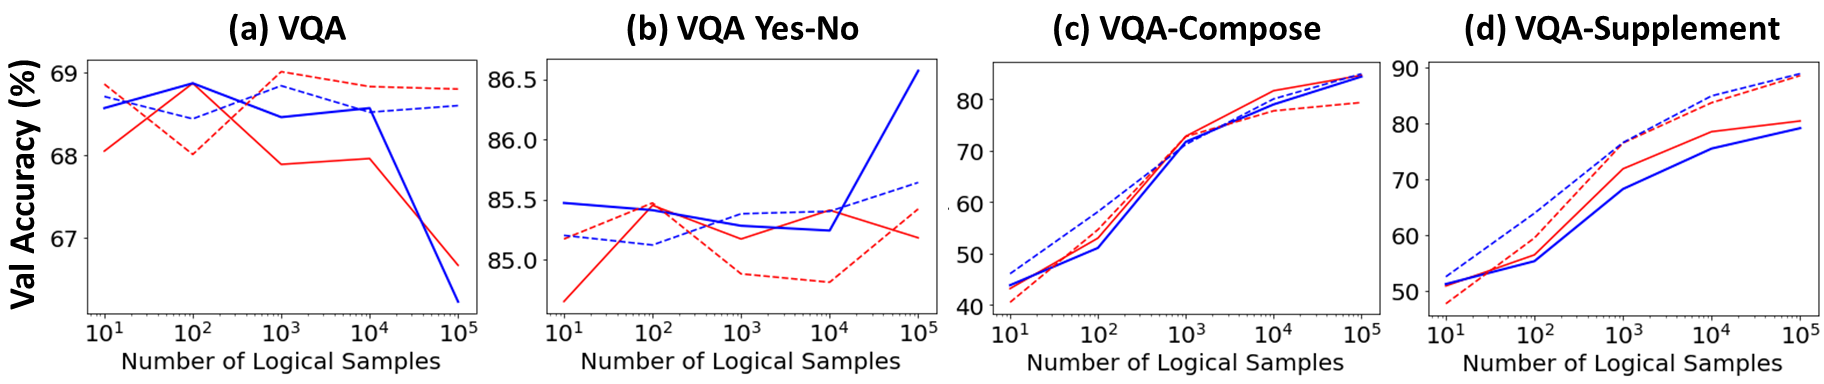
\includegraphics[width=\linewidth]{vqalol/images/fig_exp3_new.png}
    \caption{
    % Learning Curves: Red lines denote LXMERT, Blue lines denote our LOL model with $q_{\textit{ATT}}$. 
    % Models trained on VQA + \texttt{Comp} are shown in solid and those trained on VQA + \texttt{Comp} + \texttt{Supp} are in dotted lines. Best viewed in color.
    Learning Curve comparison for models (Red: LXMERT, Blue: LOL) trained on our datasets (solid lines: VQA~+~\texttt{Comp}, dotted lines: VQA~+~\texttt{Comp}~+~\texttt{Supp})
    }
    \label{fig:exp3}
\end{figure}
